


\documentclass[11pt]{amsart}

\usepackage{fancyhdr}
\usepackage{amsmath, amscd}
\usepackage{enumerate}
\usepackage{amsthm}
\usepackage{amssymb}
\usepackage[pdftex]{graphicx}
\usepackage{verbatim}
\usepackage[all]{xy}
%\usepackage{hyperref}
%\usepackage{homework}
%\usepackage[top=1.5in, bottom=1in, left=1.25in, right=1.25in]{geometry}



\newtheorem{thm}{Theorem}[section]
\newtheorem{Thm}{Theorem}[section]
\newtheorem{lem}[thm]{Lemma}
\newtheorem{res}[thm]{Result}
\newtheorem{obs}[thm]{Observation}
\newtheorem{clm}[thm]{Claim}
\newtheorem{cor}[thm]{Corollary}
\newtheorem{alg}{Algorithm}[section]
\newtheorem{prop}[thm]{Proposition}
\newtheorem{proposition}[thm]{Proposition}
\newtheorem{conj}[thm]{Conjecture}
\newtheorem{lemn}{Lemma}
\newtheorem{nothing}{}
\newtheorem{goal}{Goal}

%make xymatrix labels big
\renewcommand{\labelstyle}{\textstyle}

\newtheoremstyle{cond}{}{}{}{}{\bfseries}{.}{ }{#1 #3}
\theoremstyle{cond}
\newtheorem{cond}{Condition}



\newtheoremstyle{mystyle}{}{}{}{}{\sffamily\scshape\bfseries}{}{\newline}{\thmnote{#3}}
\theoremstyle{mystyle}
\newtheorem{mythm}{Theorem}[section]

\newtheoremstyle{mynum}{}{}{\itshape}{}{\bfseries}{.}{ }{#1 #3}
\theoremstyle{mynum}
\newtheorem{thmn}{Theorem}


\numberwithin{equation}{section}
\renewcommand{\theequation}{\thesection-\arabic{equation}}

\theoremstyle{definition}
\newtheorem{ex}[thm]{Example}
%\newtheorem{example}[thm]{Example}
\newtheorem{exer}[thm]{Exercise}
\newtheorem{defn}[thm]{Definition}
\newtheorem{rmk}[thm]{Remark}
\newtheorem{ques}[thm]{Question}

\renewcommand{\d}{\diamond}
\newcommand{\PER}{\mathrm{PER}}
\newcommand{\ph}{\varphi}
\newcommand{\ep}{\varepsilon}
\renewcommand{\L}{L}
\newcommand{\rev}{\mathrm{rev}}
\newcommand{\D}{\mathrm{D}}
\newcommand{\W}{\mathcal{W}}
\renewcommand{\P}{\mathcal{P}}
\newcommand{\V}{\mathcal{V}}
\newcommand{\vPER}{\V\mathrm{PER}}
\newcommand{\pre}{\mathrm{P}}
\newcommand{\suf}{\mathrm{S}}
\newcommand{\wt}{\widetilde}

\newcommand{\gl}{\mathfrac{gl}}

\newcommand{\bZ}{\mathbb{Z}}
\newcommand{\bQ}{\mathbb{Q}}
\newcommand{\bR}{\mathbb{R}}
\newcommand{\bN}{\mathbb{N}}
\newcommand{\bC}{\mathbb{C}}
\newcommand{\bP}{\mathbb{P}}
\newcommand{\bG}{\mathbb{G}}

\newcommand{\bbS}{\mathbb{S}}
\newcommand{\J}{\mathbb{J}}
\newcommand{\cA}{\mathcal{A}}
\newcommand{\cB}{\mathcal{B}}
\newcommand{\sC}{\mathscr{C}}
\newcommand{\sS}{\mathscr{S}}
\newcommand{\cS}{\mathcal{S}}
\newcommand{\cM}{\mathcal{M}}
\newcommand{\cN}{\mathcal{N}}
\newcommand{\cX}{\mathcal{X}}
\newcommand{\cY}{\mathcal{Y}}
\newcommand{\cZ}{\mathcal{Z}}
\newcommand{\cT}{\mathcal{T}}
\newcommand{\cF}{\mathcal{F}}
\newcommand{\sF}{\mathscr{F}}
\newcommand{\sM}{\mathscr{M}}
\newcommand{\cG}{\mathcal{G}}
\newcommand{\sG}{\mathscr{G}}
\newcommand{\cO}{\mathcal{O}}
\newcommand{\cV}{\mathcal{V}}
\newcommand{\cL}{\mathcal{L}}
\newcommand{\Cat}{\mathcal{C}}
\newcommand{\cC}{\mathcal{C}}
\newcommand{\cD}{\mathcal{D}}
\newcommand{\CR}{\mathcal{CR}}
\newcommand{\cSH}{\mathcal{SH}}
\newcommand{\cP}{\mathcal{P}}
\newcommand{\T}{\mathcal{T}}
\newcommand{\m}{\mathfrak{m}}
\newcommand{\p}{\mathfrak{p}}
\renewcommand{\O}{\mathbb{O}}
\newcommand{\X}{\mathbb{X}}
\newcommand{\bfx}{\boldsymbol{x}}
\newcommand{\bftheta}{\boldsymbol{\theta}}
\newcommand{\bfv}{\boldsymbol{v}}
\newcommand{\bfw}{\boldsymbol{w}}
\newcommand{\ada}{\textsc{AdaBoost} }
\DeclareMathOperator*{\argmin}{arg\,min}
\DeclareMathOperator*{\argmax}{arg\,max}

\newcommand{\chicon}{\chi^\circ}

\newcommand{\Hom}{{\rm Hom}}
\newcommand{\GrHom}{{\rm GrHom}}
\newcommand{\End}{{\rm End}}
\newcommand{\Func}{{\rm Func}}
\newcommand{\Spec}{{\rm Spec}} 	
\newcommand{\mSpec}{{\rm mSpec}}
\newcommand{\Bimod}{{\sf bimod}}
\newcommand{\Rep}{{\sf Rep}}
\newcommand{\Id}{{\rm Id}}
\newcommand{\id}{{\rm id}}
\newcommand{\Aut}{{\rm Aut}}
\newcommand{\GrAut}{{\rm GrAut}}
\newcommand{\supp}{{\rm Supp}}

\newcommand{\Proj}{{\rm Proj}}
\newcommand{\GL}{{\rm GL}}
\newcommand{\ann}{{\rm ann}}

\newcommand{\F}{\mathcal{F}}
\newcommand{\G}{\mathcal{G}}

\newcommand{\la}{\langle}
\newcommand{\ra}{\rangle}
\newcommand{\<}{\langle}
\renewcommand{\>}{\rangle}

\newcommand{\Ker}{{\rm Ker}}
\newcommand{\Coker}{{\rm Coker}}
\renewcommand{\Im}{{\rm Im}}
\newcommand{\coh}{{\sf coh}}
\newcommand{\Qcoh}{{\sf Qcoh}}
\newcommand{\Cont}{{\rm Cont}}
\newcommand{\tr}{{\rm tr}}

\newcommand{\xol}{\overline{x}}
\newcommand{\yol}{\overline{y}}
\newcommand{\Zol}{\overline{Z}}
\newcommand{\Phiol}{\overline{\Phi}}

\newcommand{\zv}{\ul{\theta}}


\newcommand{\Oo}{\mathcal{O}}

\def\sK{{\sf K}}
\def\per{{\rm per}}

\renewcommand{\d}{\ensuremath{\diamond}}

\newcommand{\dlim}{\lim_{\longrightarrow}}
\newcommand{\gExt}{\underline{\Ext}}
\newcommand{\gHom}{\underline{\Hom}}

\def\HPA{{\sf H}_p A}
\def\CA{{\sf C}A}
\def\HA{{\sf H}A}
\def\sC{{\sf C}}
\def\sH{{\sf H}}
\def\sD{{\sf D}}
\def\sL{{\sf L}}
\def\sX{{\sf X}}
\def\DA{{\sf D}A}
\def\Mod{{\sf Mod}}
\def\mod{{\sf mod}}
\def\add{{\sf add}}
\def\gr{\operatorname {\sf gr}}
\def\Gr{\operatorname {\sf Gr}}
\def\fdim{\operatorname {\sf fdim}}
\def\qgr{\operatorname {\sf qgr}}
\def\Qgr{\operatorname {\sf QGr}}
\def\QGr{\operatorname {\sf QGr}}
\def\Fdim{\operatorname {\sf Fdim}}
\def\Set{\operatorname {\sf Set}}
\def\Ab{\sf Ab}
\def\RM{{\sf RM}}
\def\Rings{{\sf R}}
\def\GrRep{\operatorname {\sf GrRep}}
\def\pdim{\operatorname{pdim}}
\def\gldim{\operatorname{gldim}}
\def\GK{\operatorname{GKdim}}
\def\Tor{{\rm Tor}}
\def\Ext{{\rm Ext}}
\def\rad{{\rm rad}}
\def\soc{{\rm soc}}
\def\loc{{\rm loc}}
\def\ls{\overline{\lim}}
\def\bv{\bold{v}}

\def\rk{{\rm rk}}
\def\colim{{\rm colim}}

\mathchardef\mhyphen="2D

\newcommand{\lMod}[1]{\operatorname{\mathnormal{#1}-{\sf Mod}}}
\newcommand{\rMod}[1]{\operatorname{{\sf Mod}-\mathnormal{#1}}}
\newcommand{\lmod}[1]{\operatorname{\mathnormal{#1}-{\sf mod}}}
\newcommand{\rmod}[1]{\operatorname{{\sf mod}-\mathnormal{#1}}}
\newcommand{\set}[1]{\left\{#1\right\}}
\newcommand{\ul}[1]{\underline{#1}}
\newcommand{\ol}[1]{\overline{#1}}
\newcommand{\ma}[1]{\left[\begin{matrix} #1 \end{matrix}\right]}
\newcommand{\pma}[1]{\begin{pmatrix} #1 \end{pmatrix}}
\newcommand{\bx}[1]{\noindent
\framebox[1.01\linewidth][l]{
%\framebox[0.6cm]{1.1} 
%\hfil
\parbox[t]{0.95\linewidth}{
#1
}}\\}

\renewcommand{\l}{\ell}

%beamer stuff
\newcommand{\tc}[2]{\textcolor{#1}{#2}}
\newcommand{\tcr}[1]{\textcolor{red}{#1}}
\newcommand{\bex}{\tc{blue}{Example: }}





\begin{document}

\title[]{The twitter project: my notes}
\date{\today}
\author{Gautam Sisodia} 
\maketitle

\section{To do}

\begin{itemize}
\item Migrate to MySQL, server
\end{itemize}


\section{Graph database}

\subsection{Nodes}

The nodes represent twitter users. A node has as data the user id, user name, number of friends and number of followers.

\subsection{Relationships}

There is a relationship from node $A$ to node $B$ if and only if twitter user $A$ follows twitter user $B$. 


\section{Collecting data}

\subsection{Sqlite}


\section{Hierarchy}


\subsection{The paper \cite{hier1}}

Let $G = (V, E)$ be a directed graph. Write $n = |V|$, $m = |E|$. All of the following definitions are from \cite{hier1}.

\begin{defn}
A {\bf ranking} of $G$ is a map $V \to \bN$. Denote the set of rankings of $G$ by $R(G)$.
\end{defn}

\begin{defn}
The {\bf agony} of a ranking $r \in R(G)$ is
$$
A(r) := \sum_{(u, v) \in E} \max \{ r(u) - r(v) + 1, 0\}.
$$
The hierarchy of $r$ is
$$
h(r) := 1 - (1/m)A(r).
$$ 
\end{defn}

\begin{defn}
The {\bf agony} of $G$ is
$$
A(G) := \min_{r \in R(G)}A(r),
$$
and the {\bf hierarchy} of $G$ is 
$$
h(G) := 1 - (1/m)A(G).
$$
\end{defn}

By \cite{hier1}, $A(G)$ is at most $m$, so $0 \leq h(G) \leq m$. Also, \cite{hier1} gives an $O(m^2n)$ algorithm for computing $h(G)$ and a optimal ranking, namely a ranking $r \in R(G)$ such that $h(r) = h(G)$.

\subsection{Issues with \cite{hier1}} 
\begin{enumerate}
\item The whole of the twitter data collected as of Aug 2 2014 constitutes a directed graph with 2 million vertices and 4 million arrows, so $O(m^2n)$ isn't good enough. Alternate/approximate algorithms are needed, or MapReduce techniques.
\item It bothers me that an arrow between vertices with the same ranking adds a positive amount, namely 1, to the agony of the ranking. It is perfectly natural for two people of the same social class to associate. On the other hand, there are legitimate concerns to simply removing the 1 from the definition of agony. Namely,
\begin{enumerate}
\item the trivial ranking that gives all vertices the same rank is optimal. Perhaps the total number of ranks should be a parameter.
\item the current defintion rewards finding a better ranking over settling for an ok one
\end{enumerate}
\item There may be a mistake in the paper. Consider the following graph $G$:
\begin{figure}[h]
\centering
\makebox[\textwidth][c]{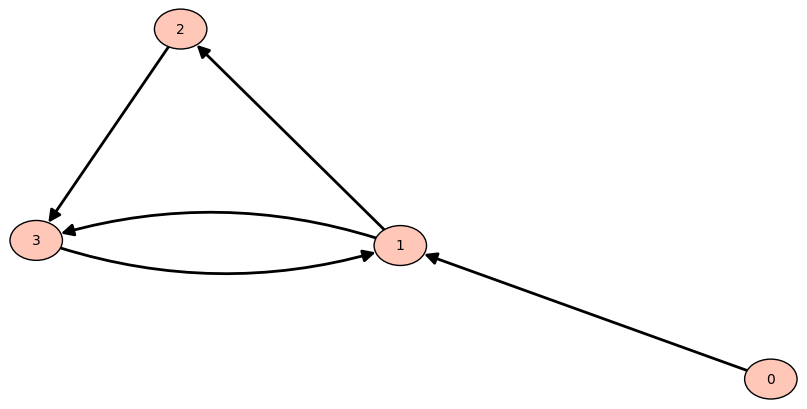
\includegraphics[width = 0.8\textwidth]{whatsgoingon}}
\caption{Bad graph?}
\label{gen}
\end{figure}
The algorithm in \cite{hier1} gives ranks 0, 1, 0, 2 to vertices 0, 1, 2, 3 respectively. This rank has agony 4 (2 from $1 \to 2$ plus 2 from $3 \to 1$). But this ranking is not optimal! The ranking 0, 1, 1, 2 has agony 3 (1 from $1 \to 2$ plus 2 from $3 \to 1$). 

UPDATE: I'm really convinced that this is actually a mistake in the paper. The mistake is at the end of Algorithm 2, when values are assigned to the integer program variables $x(i,j)$. The problem is that the values assigned may be negative, which is not feasible!

\item There is another mistake in the paper! Algorithm 2 may not (and usually doesn't) terminate! Consider the graph in figure 2. 
\begin{figure}[h]
\centering
\makebox[\textwidth][c]{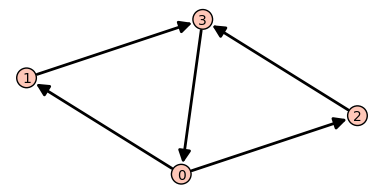
\includegraphics[width = 0.6\textwidth]{second_bad_dg}}
\caption{Another bad graph}
\label{gen}
\end{figure}
A maximal eulerian subgraph is $3 \to 0 \to 2 \to 3$. Algorithm 2 will cycle between increasing the ranks of 1, 3 and 0. 

\end{enumerate}


\subsection{Hierarchy from a difference matrix}

Here's another approach to finding a good ranking. Given two vertices $u$ and $v$ in $G$, compute somehow the best difference $r(v) - r(u)$ (probably by consider the lengths and number of paths between $u$ and $v$). Form the (non-Euclidean) difference matrix from these `distances'. Then use multidimensional scaling techniques to construct the best ranking, which leads to the next subsection. 

\subsection{Multidimensional rankings?}


\section{A stochastic gradient descent algorithm}


\begin{thebibliography}{4}


\bibitem{hier1} M. Gupte, P. Shankar, J. Li, S. Muthukrishnan, L. Iftode, {\it Social hierarchy in directed online social networks.}


\end{thebibliography}


 
\end{document}



